\chapter{\textbf{European Central Bank Speeches: A Case Study}}

Given the need to corroborate and expand research in the area of sentiment analysis applied to the economic sciences -- and based on the examples already observed in chapter \ref{chapter:lit}, an application in a case study is proposed here.\\

% In order to add something relevant to the literature, the proposed exercises work fundamentally with observable European economic variables\footnote{it is also worth mentioning the inclusion of the output gap, obtained from the Hodrick–Prescott filter \citep{hodrick1997postwar}}: -- with the exception of the proposed sentiment index (bag of words), made from two lexicons (VADER and LM-SA)

\section{Problem and Data Description}

Following the example of \cite{shapiro2020measuring}, \cite{barsky2012information} and \cite{shapiro2020measuring}, two practical exercises are proposed.\\

Firstly, in order to understand whether a sentiment index can be used for forecasting and estimating economic variables, and following the example of \cite{shapiro2020measuring}, we propose the estimation of two LASSO models (L1 norm) in order to identify possible relevant variables in scenarios macroeconomic models -- the first model is the conventional LASSO and the second the Adaptive LASSO. Still, in order to expand the field of estimations, an elastic net model is estimated, in order to capture improvements in model specifications and improve the selection of variables when the coefficients are close to zero  when:the coefficients are close to zero, elastic net tries to take advantage of the information provided by the variables without necessarily forcing the coefficients to zero, and without considering a scenario where all variables are used in order to improve a model (L2 norm).\\

From there, the estimation of an autoregressive vector (VAR) is considered, also following the indications of the literature \citep{shapiro2020measuring, barsky2012information} to better understand how a sentiment index relates to a macroeconomic scenario (and its variables). For this, the main focus of the second exercise is the exploration of impulse and response functions obtained through VAR.

The proposed exercises work fundamentally with observable European economic variables\footnote{it is also worth mentioning the inclusion of the output gap, obtained from the Hodrick–Prescott filter \citep{hodrick1997postwar}}, with the exception of the proposed sentiment index (bag of words), made from two lexicons (VADER and LM-SA).\\

The other series used for the exercises were obtained from the website of FRED - Federal Reserve Bank of St. Louis - and they are: Consumer Price Index: Harmonized Prices: Total All Items for the Euro Area; Consumer Opinion Surveys: Consumer Prices: Future Tendency of Inflation: European Commission and National Indicators for the Euro Area\footnote{Following the guidance of \cite{shapiro2020measuring}}; Real Gross Domestic Product (Euro/ECU series) for Euro area; Long-Term Government Bond Yields: 10-year: Main (Including Benchmark) for the Euro Area; Harmonized Unemployment Rate: Total: All Persons for the Euro Area. Two dummies were also included in the exercise, the first referring to the Subprime mortgage crisis; and the second referring to the economic crisis generated by the COVID-19 pandemic.\\

%\subsection{Sentiment Indexes}

Given that both series referring to sentiment indices are also not observable, they were obtained as proxies for the speeches of the European central bank\footnote{Speeches are available at https://www.ecb.europa.eu/press/key/date/html/index.en.html}. The methodology discussed here is based on \cite{loughran2011liability}, taking into account its contribution to the literature when referring to the applicability of sentiment analysis applied to economics.\\

According to \cite[p. 35]{loughran2011liability} it is possible to measure, as well as classify an economic text from the negative words in a way that the tone of these presents a correlation with economic and financial variables, since ``The results to date indicate that negative word classifications can be effective in measuring tone, as reflected by significant correlations with other financial variables''\\

As stated by \cite[p. 13]{shapiro2021taking} ``There is a large and growing literature aimed at quantifying sentiment from text. We use a method known as the `Bag of Words' or `lexical' approach, which relies on predefined dictionaries of words that are associated with particular sentiments'' -- in this work we also consider the polarity when taking into account the VADER -- analysis from valence, given a score. Unlike VADER, where the polarity is displayed\footnote{The polarity was obtained from the Natural Language Toolkit \cite[]{bird2009natural} module for Python from positive, negative, neutral and compound words.} the polarity of each text taking into account the LM-SA-2020 and extracting the composition of negative words in order to consider the weight of each term as a function of the total terms:

\begin{quote}
``In the context of information retrieval [\dots] note that term weighting `has an enormous impact on the effectiveness of a retrieval system.' Essentially, term weighting acknowledges that raw word counts are not the
best measure of a word’s information content''\cite[p. 42]{shapiro2020measuring}  
\end{quote}
So, given the occurrence of a negative word $W_{Negative}$, its frequency is computed so that the index, based on the negative terms, is given by:
\begin{align*}
I_{Negative, i} = \frac{W_{Negative, i}}{W_{Total, i}} \quad ,
\end{align*}

Where, $I_{Negative, i}$ represents the index score given the discourse $i$ of the corpus; $W_{Negative, i}$ represents the number of negative words given the speech $i$ of the corpus; and $W_{Total, i}$ represents the total number of words (positive, negative and neutral) given the speech $i$ of the corpus. As the European central bank usually carries out more than one speech per month and the objective is the value of the monthly index, it was necessary to group the values obtained per speech around its monthly average, so that:
\begin{align*}
    I_{t} = \frac{1}{n}\sum_{i=1}^{n}I_{Negative,i} \quad
\end{align*}

That is, the monthly value of the index is given by the average of the scores of the indexes of each speech in the same month.\\

The Figure \ref{fig:correlationvaderlmsa} presents the scatter plot between the two formulated indices: VADER (valence) and LM-SA-2020 (polarity). Even though the polarity calculation methodology is different for both lexicons, the Pearson correlation coefficient between them is, as expected, positive (69.76\%).

\begin{figure}[!h]
    \centering
    \caption{Correlation between the polarities obtained from the VADER and LM-SA-2020 lexicons (negative words)}
    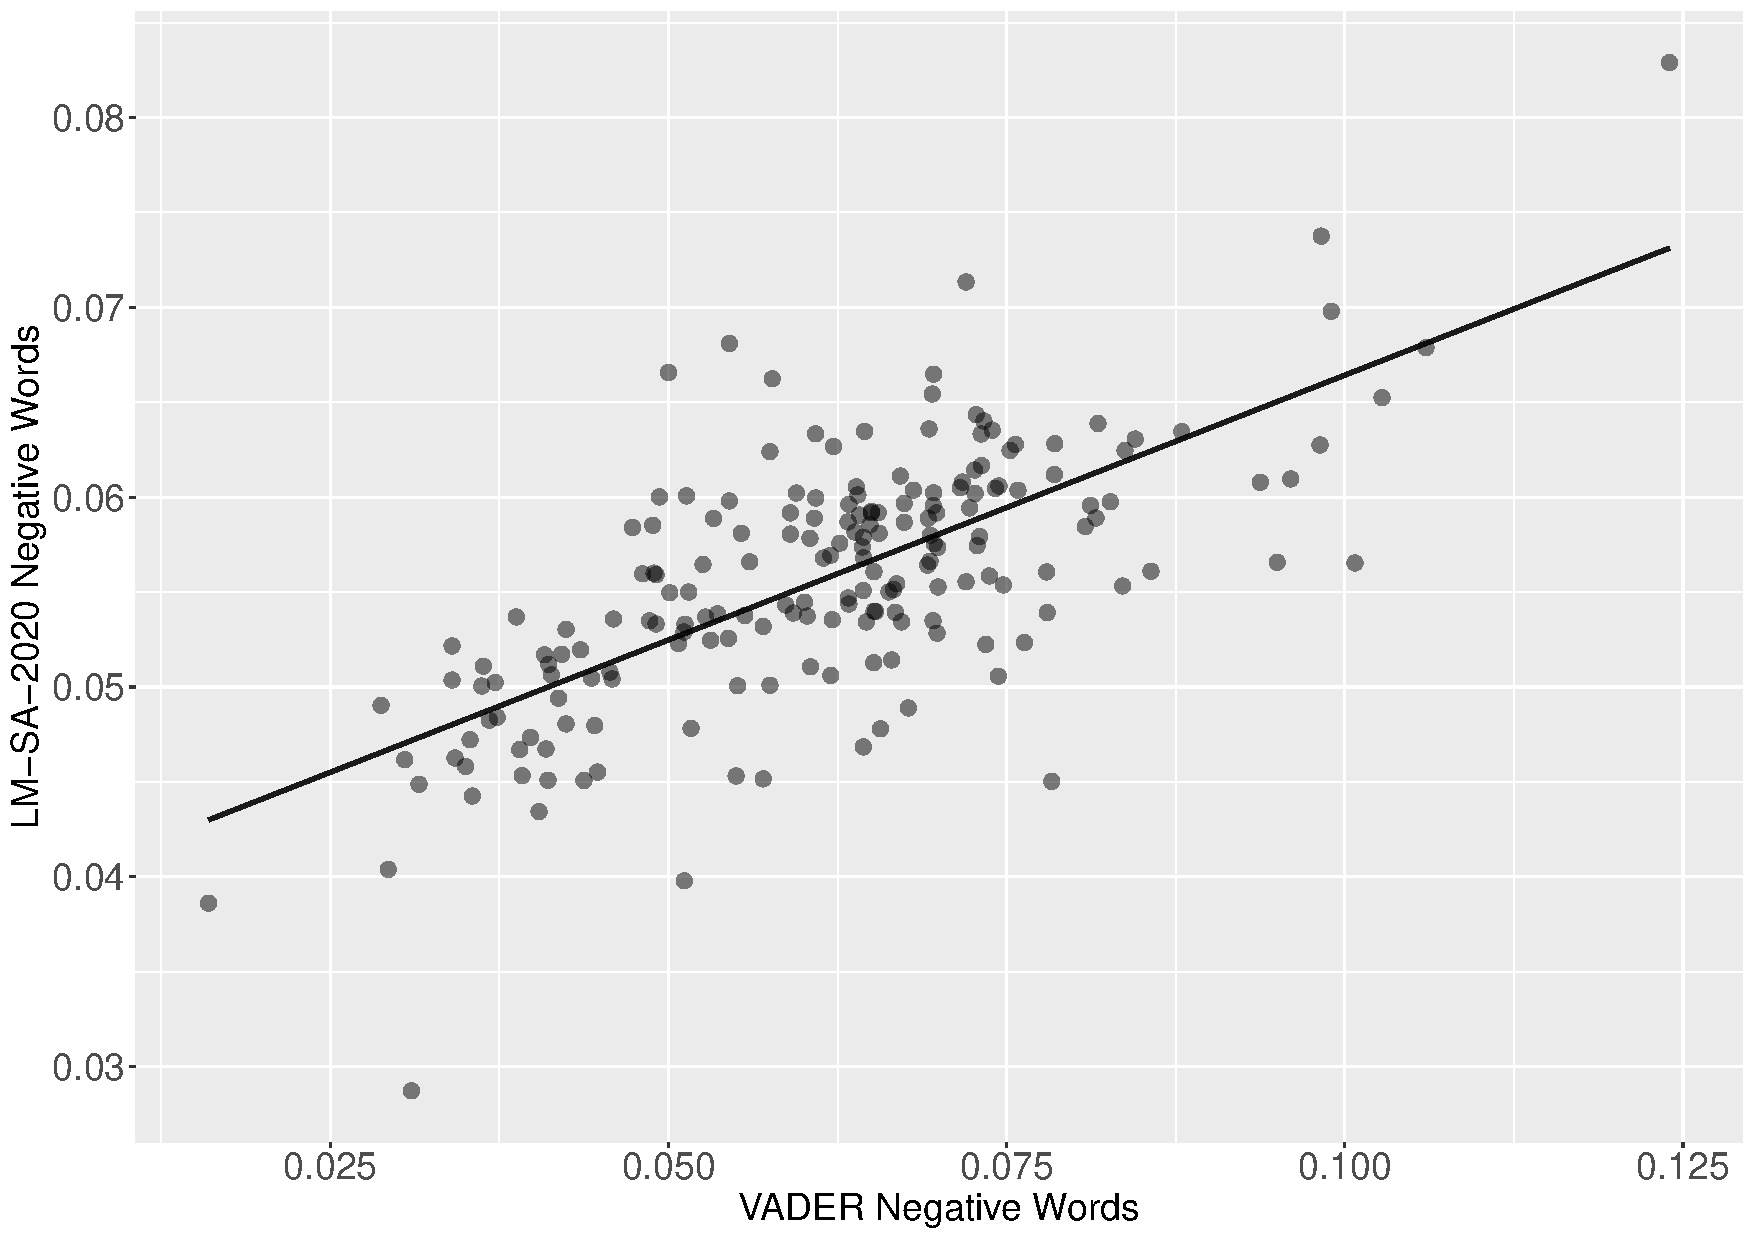
\includegraphics[width=.7\textwidth]{images/correlation_vader_lm.pdf}
    \label{fig:correlationvaderlmsa}
\end{figure}

Both indices are used in the case studies. At first, it would be recommended to \cite[p. 62]{loughran2011liability} the main use of a lexicon focused on economic and financial terms and words (LM-SA-2020) -- however, VADER is used due to the excellent results that this lexicon presents. Furthermore, it is considered an exercise to compare both lexicons: in consideration of the fact that the LM-SA-2020 focuses on economic and financial terms and words, in contrast to VADER, which, even being aimed at media analysis, has excellent results against similar lexicons.

\section{Experimental Setup}

Since the case studies consider certain statistical and econometric techniques, it is necessary to consider some assumptions in relation to the methodologies adopted and to analyze the behavior of the time series.\\

The time horizon adopted was from January 2005 to December 2020 -- it was not possible to extend this work until the year 2021 due to lack of data at the time of writing this: moreover, the choice of period was arbitrary, considering , however, the availability of the economic series and the availability of the speeches of the European Central Bank used. In all, the original database is composed of 132 observations so that two of the variables are sentiment indices (VADER and LM-SA-2020); two dummies are considered for the estimation of the variable selection models, namely: 1st- COVID, so that if the time point is February, March, or April 2020, COVID = 1, otherwise COVID = 0; 2nd - Debt Crisis in Europe, so that if the time period is from September 2011 to January 2013, the dummy assumes the value of 1, otherwise 0; all other variables are observable economic variables -- with the exception of the output gap, obtained from the Hodrick-Prescott filter.\\

In addition, it is noteworthy that, for convenience in relation to the estimations and the number of observations, it was chosen to use series of monthly frequency.\\

Also regarding the behavior of the series, two unit root tests were performed to verify the stationarity condition: the Augmented-Dickey-Fuller \cite[]{cheung1995lag} and the Phillips \& Perron Unit Root Test \cite[]{phillips1988testing} -- both were estimated from the URCA package \cite[]{urcacran} from the R software \cite[]{rcran}. Since in one of the case studies the stationarity condition is necessary for the exercise to be carried out, the series that are not zero-order I(0) integrated must be treated.\\

Basically, the Augmented-Dickey-Fuller and Phillips \& Perron tests consist of verifying whether the time series have a unit root. In the case of the Augmented-Dickey-Fuller test, given the equation:
\begin{align}
    \Delta y_t = \alpha + \beta t + \gamma y_{t-1} + \sum_{i=1}^{p} \delta_i \Delta y_{t-i} + \varepsilon_t
\end{align}
where $\alpha$ is the model constant, $\beta$ the coefficient related to the trend, $p$ is the order of the autoregressive process and $\Delta$ represents the difference in the series. If both $\alpha$ and $\beta$ are not significant for the model, that is $\alpha = 0$ and $\beta = 0$, the variation of $y$ in $t$ will be explained only by $\varepsilon$, that is, by a white noise.\\

The Phillips \& Perron unit root test, in turn, considers a model with an autoregressive process of order 1, so that:
\begin{align}
    y_t = \alpha + \beta t + \phi y_{t-1} + \varepsilon_t
\end{align}
where $\alpha$ is the model constant, $\beta$ the coefficient related to the trend, $\phi$ is the coefficient related to a first order autoregressive process and $\varepsilon$ is a white noise. Again, if $\alpha=0$ and $\beta = 0$ we are dealing with a situation where the series $y_t$ is explained only by a white noise, thus characterizing a random walk -- that is: the series is non-stationary. \\

Both tests were performed for all series, with the exception of the indices of sentiments in difference, since both indices were stationary at level, these were only tested for level. In relation to the other variables tested (Table {\ref{tab:urlevel}}), only the Product Gap (statistically significant at 1\% with trend ADF test); Producer Prices Index (statistically significant at 5\% PP test) and Interest Rate (statistically significant
at 10\% ADF) were identified as stationary. 


\begin{table}[!h]
\caption{Unit Root Tests: Augmented-Dickey-Fuller and Phillips \& Perron}
\begin{adjustbox}{max width=\textwidth}
\begin{tabular}{lllllllllll} 
\hline
                               & \multicolumn{6}{c|}{Augmented-Dickey-Fuller}                                        & \multicolumn{4}{c}{Phillips \& Perron}                    \\ \cline{2-11} 
                               & \multicolumn{2}{c|}{None} & \multicolumn{2}{c|}{Drift} & \multicolumn{2}{c|}{Trend} & \multicolumn{2}{c|}{Constant} & \multicolumn{2}{c}{Trend} \\ \hline
Consumer Opinion Surveys       & -0.69189        &         & -2.46604        &          & -2.57411        &          & -2.51257          &           & -2.59686        &         \\
Unemployment Rate              & -1.12625        &         & -0.16789        &          & -1.60657        &          & -0.12221          &           & -1.71892        &         \\
Interest Rate                  & -1.90764        & *       & -0.99368        &          & -2.52323        &          & -0.95965          &           & -2.54834        &         \\
Consumer Price Index           & -0.9864         &         & -1.16925        &          & -1.96056        &          & -1.23476          &           & -1.958          &         \\
Gap Gross Domestic Product     & 0.576651        &         & -2.03914        &          & -4.33739        & *        & -1.6031           &           & -2.97149        &         \\
Producer Prices Index          & 0.726163        &         & -3.11724        & *        & -2.92142        &          & -2.99263          & *         & -2.64357        &         \\
Negative Sentiment (VADER)     & -1.15748        &         & -7.23406        & *        & -8.13027        & *        & -9.89749          & *         & -10.5938        & *       \\
Negative Sentiment LM-SA-2020) & -0.57929        &         & -7.39231        & *        & -7.36532        & *        & -9.93006          & *         & -9.89294        & *       \\ \hline
\end{tabular}
\end{adjustbox}
\caption*{Note: * symbolizes that the series do not reject the null hypotheses of the tests, in the absence of a unit root. The test statistics, for the Augmented-Dickey-Fuller test for none, drift and trend are respectively for 10\%, 5\% and 1\%:-2.58, -1.95, -1.62; -3.46, -2.88, -2.57; -3.99, -3.43 and -3.13. For Phillips \& Perron test for constant and trend are respectively for 10\%, 5\% and 1\%: -3.48, -2.88, -2.58; -4.03, -3.44 and -3.15.}
\label{tab:urlevel}

\end{table}

In order to follow the economic literature, and with the exception of the Product Gap variable, the series are treated as difference and, thus, the unit root tests are redone\footnote{The sentiment indices and Product Gap are, therefore, , worked at level}.\\

\section{Pre-Processing Data}
In order to treat the variables in order to obtain the stationarity condition, we now proceed to treat the series in difference, since the series that are not stationary are first-order I(1) integrated, we work with the series from the first difference.\\

When running the tests in difference all series, both tests reject the null hypothesis of unit root at 1\% (Table \ref{tab:urdiff}). The need to verify the stationarity condition becomes essential for one of the proposed case studies: the estimation of an Vector Autoregressive is not possible if any of the variables does not fulfill this condition.


% --------------------------------------------------

\begin{table}[!h]
\caption{Unit Root Tests for the Series in Difference: Augmented-Dickey-Fuller and Phillips \& Perron}
\begin{adjustbox}{max width=\textwidth}
\begin{tabular}{lllllllllll}
\hline
                           & \multicolumn{6}{c|}{Augmented-Dickey-Fuller}                                        & \multicolumn{4}{c}{Phillips \& Perron}                    \\
                           & \multicolumn{2}{c|}{None} & \multicolumn{2}{c|}{Drift} & \multicolumn{2}{c|}{Trend} & \multicolumn{2}{c|}{constant} & \multicolumn{2}{c}{trend} \\ \hline
Consumer Opinion Surveys   & -7.38867        & *       & -7.36197        & *        & -7.37293        & *        & -9.22024          & *         & -9.2483         & *       \\
Unemployment Rate          & -4.59511        & *       & -4.65701        & *        & -4.78258        & *        & -7.60278          & *         & -7.70628        & *       \\
Interest Rate              & -7.35245        & *       & -7.56178        & *        & -7.53145        & *        & -9.97176          & *         & -9.9337         & *       \\
Consumer Price Index       & -7.03739        & *       & -7.04257        & *        & -7.03008        & *        & -11.1771          & *         & -11.2587        & *       \\
Gap Gross Domestic Product & -6.87391        & *       & -6.9118         & *        & -6.89305        & *        & -6.57819          & *         & -6.55389        & *       \\
Producer Prices Index      & -6.07706        & *       & -6.11674        & *        & -6.21462        & *        & -6.08898          & *         & -6.19294        & *       \\ \hline
\end{tabular}
\end{adjustbox}
\caption*{Note: * symbolizes that the series do not reject the null hypotheses of the tests, in the absence of a unit root. The test statistics, for the Augmented-Dickey-Fuller test for none, drift and trend are respectively for 10\%, 5\% and 1\%:-2.58, -1.95, -1.62; -3.46, -2.88, -2.57; -3.99, -3.43 and -3.13. For Phillips \& Perron test for constant and trend are respectively for 10\%, 5\% and 1\%: -3.48, -2.88, -2.58; -4.03, -3.44 and -3.15.}
\label{tab:urdiff}
\end{table}

Given that the series are stationary in difference, for the VAR case study, we will use them like this, for the other exercise the series will remain level.

\section{Modeling}

Two exercises are proposed, as previously mentioned. First, a case study will be carried out taking into account the inclusion of sentiment indices when considering economic models when utilizing Variable Selection Models criteria. For this, the LASSO, Adaptive LASSO and Elastic Net models are used.\\

The second case study refers to an Autoregressive Vector (VAR) -- impulse response functions are used to better understand the behavior of macroeconomic variables when a shock is given to one of the sentiment indices (VADER and LM- SA-2020).\\

\subsection{Variable Selection Models}

Variable selection models have as main objective the identification and statistically significant variables for a model. Unlike information criteria such as AIC \cite[]{akaike1974new} and BIC \cite[]{schwarz1978estimating}, the variable selection models used here are variations of the conventional LASSO model. That is, the selection of variables is done by forcing the coefficients related to each variable to 0 when not significant, so that when significant, the coefficients are greater than 0.\\

The first method of Variable Selection Models used in this first case study is the conventional LASSO. The LASSO estimator (least absolute shrinkage and selection operator) is a linear estimation method presented in 1996 in a paper entitled ``Regression Shrinkage and Selection via the lasso'' \cite[]{tibshirani1996regression}. For regressions and generalized regressions, this estimator was proposed as a shrinkage and selection method.\\

Assuming a data set such that $(x^i, y_i)$ and $i = 1, 2, \dots , N$, and assuming $x^i = (x_{i1}, \dots, x_{ip})^T$ are the predictor variables and $y_i$ is the dependent variable. Also, since $\hat{\beta} = (\beta_1, \dots, \beta_p)^T$ the estimate LASSO $(\hat{\beta}^{lasso})$ \cite[p. 268]{tibshirani1996regression} is given in its Lagrangian equivalent by:

\begin{align} \label{eq:lasso}
    \hat{\beta}^{lasso} = \frac{1}{2}(y - Xb)'(y - Xb) + \lambda\sum_{j=1}^p|b_j|
\end{align}
the penalty on $\sum_1 ^p |\beta_j|$ is called the L1 lasso penalty \cite[p.68]{hastie2009elements} and this last constraint makes the solution nonlinear in $y_i$. The LASSO, however, ``does not focus on subsets but rather defines a continuous shrinking operation that can produce coefficients that are exactly 0''\cite[p.286]{tibshirani1996regression}. Thus, it can be seen that the greater $\lambda$, the greater the number of coefficients defined as 0. The value of $\lambda$ in this case study is obtained by cross validation following the literature\cite[p. 136]{hoornweg2018science}.\\

Another estimator used in this case study as a variable selection model is the first variation of the LASSO presented here. The  Adaptive lasso estimator was first described by \cite{zou2006adaptive} and, in contrast to lasso, augments the penalty with a vector of weights. The adaptive LASSO estimator ($\hat{\beta}^{alasso}$), then, is given by:

\begin{align} \label{eq:lassoadaptive}
    \hat{\beta}^{alasso} = \frac{1}{2}(y - Xb)'(y - Xb) + \lambda\sum_{j=1}^p\hat{w}_j |b_j|
\end{align}

Where $\hat{w}_j$ is a vector of weights and can ``be given by $\hat{w}_j = \frac{1}{|b_{ols, j}|^\gamma}$, for some $ \gamma > 0$'' \cite[p. 115]{hoornweg2018science}.\\

The third variable selection model used here is the Elastic Net model \cite[]{zou2005regularization}. Despite the fact that there are more choices for other LASSO models, like the random LASSO \cite[]{wang2011random} and the group LASSO \cite[]{yuan2006model}, Elastic Net was used for being a well-known reference in the literature and for combining the L2 penalty\footnote{The L2 penalty is also known as Ridge regression \cite[p.2]{owen2007robust}.}:

\begin{align}\label{eq:elasticnet}
    \hat{\beta}^{enet} = \frac{1}{2}(y - Xb)'(y - Xb) + \lambda\sum_{j=1}^p\left(\frac{\alpha}{2}b_j ^2 + (1 - \alpha)|b_j|\right)
\end{align}
The formulation presented in (\ref{eq:elasticnet}) is the same formulation presented by \cite{hastie2009elements}. The Elastic Net model introduces a parameter $\alpha$ into the model so that when $\alpha = 0$ the model only incorporates the L1 LASSO penalty; and when $\alpha = 1$ the model only incorporates the L2 Ridge penalty; when $0 < \alpha < 1$ the Elastic Net model incorporates properties from both the LASSO model and the Ridge model. In this case, both $\lambda$ and $\alpha$ were obtained from cross validation.


\subsection{Vector Autoregression}

In order to consider a deeper analysis in terms of economic simulation, and taking into account the endogeneity characteristic, a Vector Autogression (VAR) model is estimated as a second case study. In mathematical terms, we can represent a VAR(1) in a matrix form, that is, a first-order Autoregressive Vector as follows:

\begin{align} \label{eq:var1}
    \begin{bmatrix}
    y_{1,t} \\
    y_{2,t}
    \end{bmatrix} = 
    \begin{bmatrix}
    \delta_1\\
    \delta_2
    \end{bmatrix} +
    \begin{bmatrix}
    \phi_{11} & \phi_{12} \\
    \phi_{21} & \phi_{22}
    \end{bmatrix}
    \begin{bmatrix}
    y_{1,t-1} \\
    y_{2,t-1}
    \end{bmatrix} +
    \begin{bmatrix}
    \varepsilon_{1,t} \\
    \varepsilon_{2,t}
    \end{bmatrix} 
\end{align}

Where $y_1$ and $y_2$ are endogenous variables and $\varepsilon_1$ and $\varepsilon_2$ are the error terms for each equation. $\phi_{12}$ represents, in turn, the linear dependence of $Y_{1, t}$ on $y_{2, t-1}$ given the presence of $y_{1, t-1}$ . Thus, if $\phi_{12} = 0$, then $y_{1, t}$ does not depend on $y_{2, t-1}$ when $y_{2, t-1}$ is given. \\

Also, according to \cite{verbeek2008guide}, we can represent a first-order Autoregressive Vector as follows:

\begin{align*}
    \overrightarrow{Y_t} = \phi + \theta \overrightarrow{Y_{t-1}} + \overrightarrow{\varepsilon_t} \quad ,
\end{align*}
where, for a VAR(1) with two variables: $\overrightarrow{Y_t} = [y_{1,t}, y_{2, t}]'$ and $\overrightarrow{\varepsilon_t} = [\varepsilon_{1, t}, \varepsilon_{2, t}]$. Thus, in general a VAR(P) can be written as follows:

\begin{align*}
    \overrightarrow{Y_t} = \phi + \theta_1 \overrightarrow{Y_{t-1}} + \dots + \theta_p \overrightarrow{Y_{t-p}} + \overrightarrow{\varepsilon_t} \quad ,
\end{align*}
where each $\theta_j$ is a matrix $k \times k$ and $\overrightarrow{\varepsilon_t}$ is a vector of length $k$ of white noises, with a covariance matrix defined by $\sum$.\\

For each of its parts, the VAR model implies an ARMA model. Since the information set is expanded to additionally include the history of other variables, evaluating the components simultaneously has the advantages of being more parsimonious, containing fewer lags, and allowing for more accurate predictions \cite[p.322]{verbeek2008guide}. From a different angle, \cite{sims1980macroeconomics} asserts that using VAR models rather than simultaneous structural equations is advantageous since no 'arbitrary' limitations or previous assumptions need to be made regarding the separation between exogenous and endogenous variables.\\

In the same way that we can represent an Autoregressive from its moving average component, we can also write a VAR as a moving average vector. Considering the equation (\ref{eq:var1}, we can represent it as follows:

\begin{align} \label{eq:mavar1}
    \begin{bmatrix}
    y_{1,t} \\
    y_{2,t}
    \end{bmatrix} = 
    \begin{bmatrix}
    \bar{y_1}\\
    \bar{y_2}
    \end{bmatrix} + \sum_{i=0}^{\infty}
    \begin{bmatrix}
    \phi_{11} & \phi_{12} \\
    \phi_{21} & \phi_{22}
    \end{bmatrix}^i
    \begin{bmatrix}
    \varepsilon_{1,t-i} \\
    \varepsilon_{2,t-i}
    \end{bmatrix} 
\end{align}
Where $y_{1, t}$ and $y_{2, t}$ are expressed in terms of \{$\varepsilon_{1, t}$\} and \{$\varepsilon_{1, t}$\} respectively. According to \cite{enders2008applied}, it is possible to rewrite the previous equation in terms of \{$\varepsilon_{y1, t}$\} and \{$\varepsilon_{y2, t}$\}. Thus, the error vector can be written as follows:

\begin{align} \label{eq:varvarepsilon}
    \begin{bmatrix}
    \varepsilon_{1,t} \\
    \varepsilon_{1,t}
    \end{bmatrix} = \frac{1}{1 - b_{12}b_{21}}
    \begin{bmatrix}
    1 & -b_{12} \\
    -b_{21} & 1
    \end{bmatrix}
    \begin{bmatrix}
    \varepsilon_{y1, t} \\
    \varepsilon_{y2, t}
    \end{bmatrix}
\end{align}
combining the equations (\ref{eq:mavar1}) and (\ref{eq:varvarepsilon}), we obtain:

\begin{align*}
    \begin{bmatrix}
    y_{1,t} \\
    y_{2,t}
    \end{bmatrix} =
    \begin{bmatrix}
    \bar{y_1}\\
    \bar{y_2}
    \end{bmatrix} + \frac{1}{1 - b_{12}b_{21}} \sum_{i=0}^{\infty}
    \begin{bmatrix}
    \phi_{11} & \phi_{12} \\
    \phi_{21} & \phi_{22}
    \end{bmatrix}^i
    \begin{bmatrix}
    1 & -b_{12} \\
    -b_{21} & 1
    \end{bmatrix}
    \begin{bmatrix}
    \varepsilon_{y1, t} \\
    \varepsilon_{y2, t}
    \end{bmatrix} \quad ,
\end{align*}
replacing the matrix $2 \times 2$ with a generic term to simplify the notation:

\begin{align}
    \Gamma_i = \frac{A_1 ^i}{1 - b_{12}b_{21}}\begin{bmatrix}
    1 & -b_{12}\\
    -b_{21} & 1
    \end{bmatrix}
\end{align}
therefore, the moving media representation presented in (\ref{eq:mavar1}) and (\ref{eq:varvarepsilon}) can be expressed as:

\begin{align} \label{eq:mavar1}
    \begin{bmatrix}
    y_{1,t} \\
    y_{2,t}
    \end{bmatrix} = 
    \begin{bmatrix}
    \bar{y_1}\\
    \bar{y_2}
    \end{bmatrix} + \sum_{i=0}^{\infty}
    \begin{bmatrix}
    \Gamma_{11}(i) & \Gamma_{12}(i) \\
    \Gamma_{21}(i) & \Gamma_{22}(i)
    \end{bmatrix}^i
    \begin{bmatrix}
    \varepsilon_{y1, t} \\
    \varepsilon_{y2, t}
    \end{bmatrix} \quad ,
\end{align}
or in a more compact form:

\begin{align*}
    x_t = \epsilon + \sum_{i=0}^{\infty}\Gamma_i \varepsilon_{t-1}
\end{align*}
In terms of analysis, the final equation offers a very helpful tool to look at how the variables $y_1$ and $y_2$ interact with one another. For time periods of $y_1$ and $y_2$, the effects of $\varepsilon_{y1, t}$ on shocks of $\varepsilon_{y1, t}$ can be generated using the coefficients of $\Gamma_i$. As a result, it is clear that the four components of $\Gamma_{jk}(0)$ are effect multipliers \cite[p.295]{enders2008applied}.\\

By correctly adding the coefficients of the \textit{impulse response functions}, it is possible to determine the overall effects of an impulse on $\varepsilon_{y1, t}$ and/or $\varepsilon_{y2, t}$. For instance, we can observe that the impact of $\varepsilon_{y2, t}$ on the value of $y_{1+n}$ after $n$ periods is $\Gamma_{12}(n)$. The cumulative sum of $\varepsilon_{y2, t}$ effects on $y_1$ after n periods is as follows:

\begin{align*}
    \sum_{i=0}^{n}\Gamma_{12}(i) \quad ,
\end{align*}
if $y_1$ and $y_2$ are stationary, the values of $\Gamma_{jk}(i)$ converge to zero, the larger $i$ is. Shocks cannot, therefore, permanently alter stationary series. Thus, it follows:

\begin{align*}
    \sum_{i=0}^{\infty}\Gamma^2 _{jk}(i) \text{ is finite,}
\end{align*}
the four sets of coefficients $\Gamma_{11}(i)$, $\Gamma_{12}(i)$, $\Gamma_{21}(i)$ and $\Gamma_{22}(i)$ are called the impulse response function.

\section{Cross Validation and Learning Algorithms}

Cross Validation is a technique widely described in the literature \cite[]{hoornweg2018science, hastie2009elements, stone1974cross, breiman1992submodel} that aims to obtain optimal parameters from a predefined model. In Cross Validation, the dataset is divided between a training dataset and a test dataset, these being composed of 80\% and 20\% of the original dataset \cite[291]{breiman1992submodel}. The model, then, ``is estimated with a training sample and these estimates are used to ‘predict’ the outcomes of the validation sample. By varying the choice of a tuning parameters, one can select the set of configurations that leads to the best pseudo-out-of-sample forecasts''\cite[p.136]{hoornweg2018science}.\\

\begin{figure}[!h]
    \centering
    \caption{Cross Validation Flowchart}
    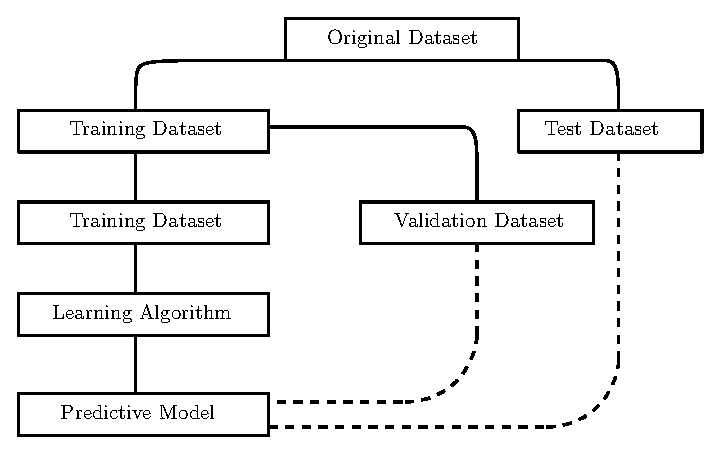
\includegraphics[width=.6\textwidth]{images/validation.eps}
    \label{fig:cv}
\end{figure}


Figure \ref{fig:cv} presents a flowchart explaining how Cross Validation works. The same procedure was performed for the models estimated in this work (LASSO, Adaptive LASSO, and Elastic Net). Both the training, validation, and test dataset division were done randomly using the texttt{Matrix} \cite[]{matrix2020cran} package of the R software.\\

Four evaluation metrics criteria were taken into consideration when performing the cross validation procedure for the variable selection models. The $R^2$ \cite{heinisch1962steel}, the MAE \cite{willmott2005advantages}, the MSE \cite{bickel2015mathematical}, and the RMSE \cite{hyndman2006another}. Based on these criteria, the values of $\lambda$ were selected for the LASSO and Adaptive LASSO models, and the values of $\lambda$ and $\alpha$ for the Elastic Net model. For the VAR models, in addition to the AIC and BIC selection criteria, the Hannan–Quinn information criterion \cite{hannan1979determination} was also used.\\

From there, the selected models were analyzed and the results will be presented in the next  section  \ref{sec:expresults}.

\section{Experimental Results} \label{sec:expresults}

Two exercises were performed in this section. First, the variable selection models are analyzed, and then in the second part of the section, the impulse response of the VAR models is analyzed. The R software and the Python language \cite[]{van1995python} were used to carry out this work, the codes can be found at \href{https://github.com/gustavovital/Dissertation}{Repository of this Dissertation}\\

\subsection{Variable Selection Models}

The first case study presented here concerns the estimation of three variable selection models, namely LASSO, Adaptive LASSO and Elastic Net\footnote{The calculations and estimations were made using the package \texttt{glmnet} \cite[] {glmnet2011noah}.}. The specification of the estimated model takes into account the addition of contemporary variables and a one-year lag in relation to the regressors and the response variable. The only variables that were not considered dependent variables in this study were the sentiment indices (VADER and LM-SA-2020) and the control dummies used (Subprime mortgage crisis and COVID-19 pandemic).\\

The optimal values of the $\lambda$ and $\alpha$ parameters were obtained through Cross Validation. First, the dataset was divided between training dataset and test dataset and, finding the optimal values of the parameters, the model was evaluated against the test dataset -- from evaluation metrics such as MAE, MSE, and RMSE it is possible to identify of the best models, among the variable selection models.\\

For the estimation of models and ``given that the LASSO model need not be parsimonious''\cite[p. 25]{shapiro2020measuring}, all series presented here were used in the model. So the LASSO\footnote{The model presented is the same for the Adaptive LASSO and Elastic Net models, only the penalty of each model changes, according to the specificity of each one.} equation (\ref{eq:lasso}) for representation purposes can be expressed as:

\begin{align}
    \hat{\beta}^{lasso} = \argmin \sum_{i=1}^{n}\left(y_{i,t+12} - \sum_{j=1}^{p}x_{i,j}b_j\right)^2 +\lambda\sum_{j=1}^p |b_j|
\end{align}
where $y_{i,t+12}$ represents the interest variable $i$ for a period of time $t+12$. In addition to the series initially presented by \cite{barsky2012information} and with the exception of the consumption series, we introduce in this study a proxy for unemployment \cite[]{shapiro2020measuring}, and the Consumer Opinion Surveys, as in the model presented by \cite{shapiro2020measuring}. Thus, $x_{i,j}$ represents the series $i$ with its respective value in the periods $t$ and $t+12$. If the variable selection models select one of the sentiment indices (VADER or LM-SA-2020), then this is an indication that the indices would help in out-of-sample predictions.\\

Table \ref{tab:selectionvader} and Table \ref{tab:selectionlm} present the selections of variables in each of the models, taking into account that each of the Tables presents one of the sentiment indices as a regression variable. In relation to Table \ref{tab:selectionvader}, it is possible to verify that the sentiment index based on VADER is not significant when in a conventional LASSO model, in terms of unemployment estimation. Even so, when considering the estimations of the Adaptive LASSO and Elastic Net models, the sentiment index based on VADER presents a coefficient different from zero. \\

In terms of evaluation metric, when considering the VADER model where the dependent variable is unemployment, the smallest MAE found was that of the Elastic Net model, with a value of 0.2071393, in contrast to the value of the LASSO model, 0.209345; in relation to the MSE, the lowest was that of the Adaptive LASSO model, with a value of 0.06461785, in contrast to the LASSO, whose value was 0.0754084; finally, when we consider the RMSE metric evaluation, the lowest value obtained was that of the Adaptive LASSO model, with a value of 0.2542004, and the conventional LASSO value was 0.2746059. Thus, it is still possible to argue in relation to the choice of model, since, when considering the metric evaluation criteria, both the Adaptive LASSO and Elastic Net models proved to be superior to the estimated conventional LASSO model, considering that among the analyzed criteria the models that maintained the VADER sentiment index stood out better in relation to the model with the exclusion of the sentiment index.\\

When comparing the three models estimated in relation to the VADER sentiment index in this study, it is possible to notice that the results are in line with the results aligned with the literature. In the models estimated by \cite{shapiro2020measuring}, when unemployment is considered as a dependent variable, only the LASSO model does not exclude the index developed by the author as an important variable in the model. The other two models estimated by the author, Adaptive LASSO and Group Lasso, end up not including this variable in the model\footnote{For clarification, when analyzing the models in which the dependent variable is ``Consumption'', these also did not select the sentiment indices developed by the author.}.\\

When analyzing Table \ref{tab:selectionlm}, the results are better. The LM-SA-2020 sentiment index as a regressor variable is present in all estimated models, LASSO, Adaptive LASSO and Elastic Net.\\

If comparing the evaluation metrics for each analyzed model (VADER and LM-SA-2020), the results are as follows: with the VADER sentiment index as a regressor variable, the best predictive model for Consumer Opinion Surveys was LASSO, for the Unemployment Rate was Adaptive LASSO, for the Interest Rate it was LASSO, for the Consumer Price Index it was LASSO, for the Gross Domestic Product it was Adaptive LASSO, and finally for the Producer Prices Index it was also the Adaptive LASSO.\\

On the other hand, when the reference regressor variable is the LM-SA-2020 sentiment index, for the Consumer Opinion Surveys, the best model analyzed was Elastic Net, for the Unemployment Rate, it was LASSO, for Interest Rate was the Adaptive LASSO, for the Consumer Price Index the LASSO and for both the Gross Domestic Product and the Producer Prices Index, the models chosen were the Adaptive LASSO.\\

When comparing the models with each other, that is, the models where one has the VADER sentiment index as a regressor variable and the other has the LM-SA-2020 sentiment index as a regressor variable, the models that had the VADER sentiment index slightly outperformed the models whose regression variable was the LM-SA-2020 sentiment index. The only model where the metric evaluation methods did not point out incisively was in relation to the model where the predictor variable was Consumer Opinion Surveys. With the exception of this one, the evaluation metrics indicated that the VADER index performed better on the following models with the following predictor variables: Unemployment Rate, Interest Rate and Gross Domestic Product. The LM-SA-2020 sentiment index stood out when the analyzed models had the following series as predictor variables: Consumer Price Index and Producer Prices Index.\\

In general, the models proved to be significant to highlight the functionality of how an economic sentiment index affects macroeconomic variables. Both indices showed significant for the estimation of the study variables in at least one of the models, LASSO, Adaptive LASSO or Elastic Net. The results obtained also corroborate the economic literature presented in this work. It is then analyzed how the economic variables would respond to a shock in sentiment indices.

\begin{landscape}
\begin{table}[]
\caption{Variable Selection Models: VADER Sentiment}
\label{tab:selectionvader}
\begin{adjustbox}{max width=\linewidth}
\begin{tabular}{llllllllll}
\hline
                         & \multicolumn{3}{c}{Consumer Opinion   Surveys} & \multicolumn{3}{c}{Unemployment Rate}      & \multicolumn{3}{c}{Interest Rate}         \\
                         & Lasso     & Adaptive Lasso    & Elastic Net    & Lasso    & Adaptive Lasso   & Elastic Net  & Lasso   & Adaptive Lasso   & Elastic Net  \\
Consumer Opinion Surveys & x         &                   & x              & x        &                  & x            & x       & x                & x            \\
Unemployment Rate        & x         & x                 & x              & x        & x                & x            & x       & x                & x            \\
Interest Rate            & x         & x                 & x              &          &                  & x            & x       & x                & x            \\
Consumer Price Index     & x         & x                 & x              & x        & x                & x            & x       & x                & x            \\
Gross Domestic Product   & x         &                   & x              &          & x                & x            & x       & x                & x            \\
Producer Prices Index    & x         & x                 & x              & x        & x                & x            & x       & x                & x            \\ \hline
VADER Sentiment          & x         & x                 & x              &          & x                & x            & x       & x                & x            \\ \hline
                         & \multicolumn{3}{c}{Consumer Price Index}       & \multicolumn{3}{c}{Gross Domestic Product} & \multicolumn{3}{c}{Producer Prices Index} \\
                         & Lasso     & Adaptive Lasso    & Elastic Net    & Lasso    & Adaptive Lasso   & Elastic Net  & Lasso   & Adaptive Lasso   & Elastic Net  \\
Consumer Opinion Surveys & x         & x                 &                & x        &                  & x            & x       & x                & x            \\
Unemployment Rate        &           &                   & x              & x        & x                & x            & x       & x                & x            \\
Interest Rate            & x         & x                 & x              & x        & x                & x            & x       & x                & x            \\
Consumer Price Index     &           &                   & x              &          & x                & x            & x       & x                & x            \\
Gross Domestic Product   &           &                   & x              &          &                  & x            & x       & x                & x            \\
Producer Prices Index    & x         & x                 & x              & x        & x                & x            & x       & x                & x            \\ \hline
VADER Sentiment          & x         & x                 & x              & x        & x                & x            & x       & x                & x \\ \hline    
\end{tabular}
\end{adjustbox}
\caption*{Note: the checkmarks symbolize that at least one of the regressors (contemporary or 12 lags) was estimated with non-zero coefficients by the LASSO, Adaptive LASSO or Elastic Net estimator indicated by the column headers. The dependent variable for each model is listed above the column headings.}
\end{table}
\end{landscape}



\begin{landscape}


\begin{table}[]
\caption{Variable Selection Models: LM-SA-2020 Sentiment}
\label{tab:selectionlm}
\begin{adjustbox}{max width=\linewidth}
\begin{tabular}{llllllllll}
\hline
                         & \multicolumn{3}{l}{Consumer Opinion Surveys} & \multicolumn{3}{l}{Unemployment Rate}      & \multicolumn{3}{l}{Interest Rate}         \\
                         & Lasso    & Adaptive Lasso    & Elastic Net   & Lasso    & Adaptive Lasso   & Elastic Net  & Lasso   & Adaptive Lasso   & Elastic Net  \\
Consumer Opinion Surveys & x        &                   & x             & x        &                  & x            & x       & x                & x            \\
Unemployment Rate        & x        & x                 & x             & x        & x                & x            & x       & x                & x            \\
Interest Rate            & x        & x                 & x             &          &                  & x            & x       & x                & x            \\
Consumer Price Index     & x        & x                 & x             &          & x                & x            & x       & x                & x            \\
Gross Domestic Product   & x        &                   & x             & x        & x                & x            & x       & x                & x            \\
Producer Prices Index    & x        & x                 & x             &          & x                & x            & x       & x                & x            \\ \hline
LM-SA-2020 Sentiment          & x        & x                 & x             & x        & x                & x            & x       & x                & x            \\ \hline
                         & \multicolumn{3}{l}{Consumer Price Index}     & \multicolumn{3}{l}{Gross Domestic Product} & \multicolumn{3}{l}{Producer Prices Index} \\
                         & Lasso    & Adaptive Lasso    & Elastic Net   & Lasso    & Adaptive Lasso   & Elastic Net  & Lasso   & Adaptive Lasso   & Elastic Net  \\
Consumer Opinion Surveys & x        & x                 & x             & x        &                  & x            & x       & x                & x            \\
Unemployment Rate        &          &                   &               & x        & x                & x            & x       & x                & x            \\
Interest Rate            & x        & x                 & x             & x        & x                & x            & x       & x                & x            \\
Consumer Price Index     &          &                   &               &          &                  & x            & x       & x                & x            \\
Gross Domestic Product   &          &                   & x             &          &                  & x            & x       & x                & x            \\
Producer Prices Index    & x        & x                 & x             & x        & x                & x            & x       & x                & x            \\ \hline
LM-SA-2020 Sentiment          & x        & x                 & x             & x        & x                & x            & x       & x                & x    \\ \hline     
\end{tabular}
\end{adjustbox}
\caption*{Note: the checkmarks symbolize that at least one of the regressors (contemporary or 12 lags) was estimated with non-zero coefficients by the LASSO, Adaptive LASSO or Elastic Net estimator indicated by the column headers. The dependent variable for each model is listed above the column headings.}
\end{table}
\end{landscape}

\begin{figure}
    \centering
    \caption{Impulse Response of a Sentiment Index (VADER) Shock on Economic Activity}
    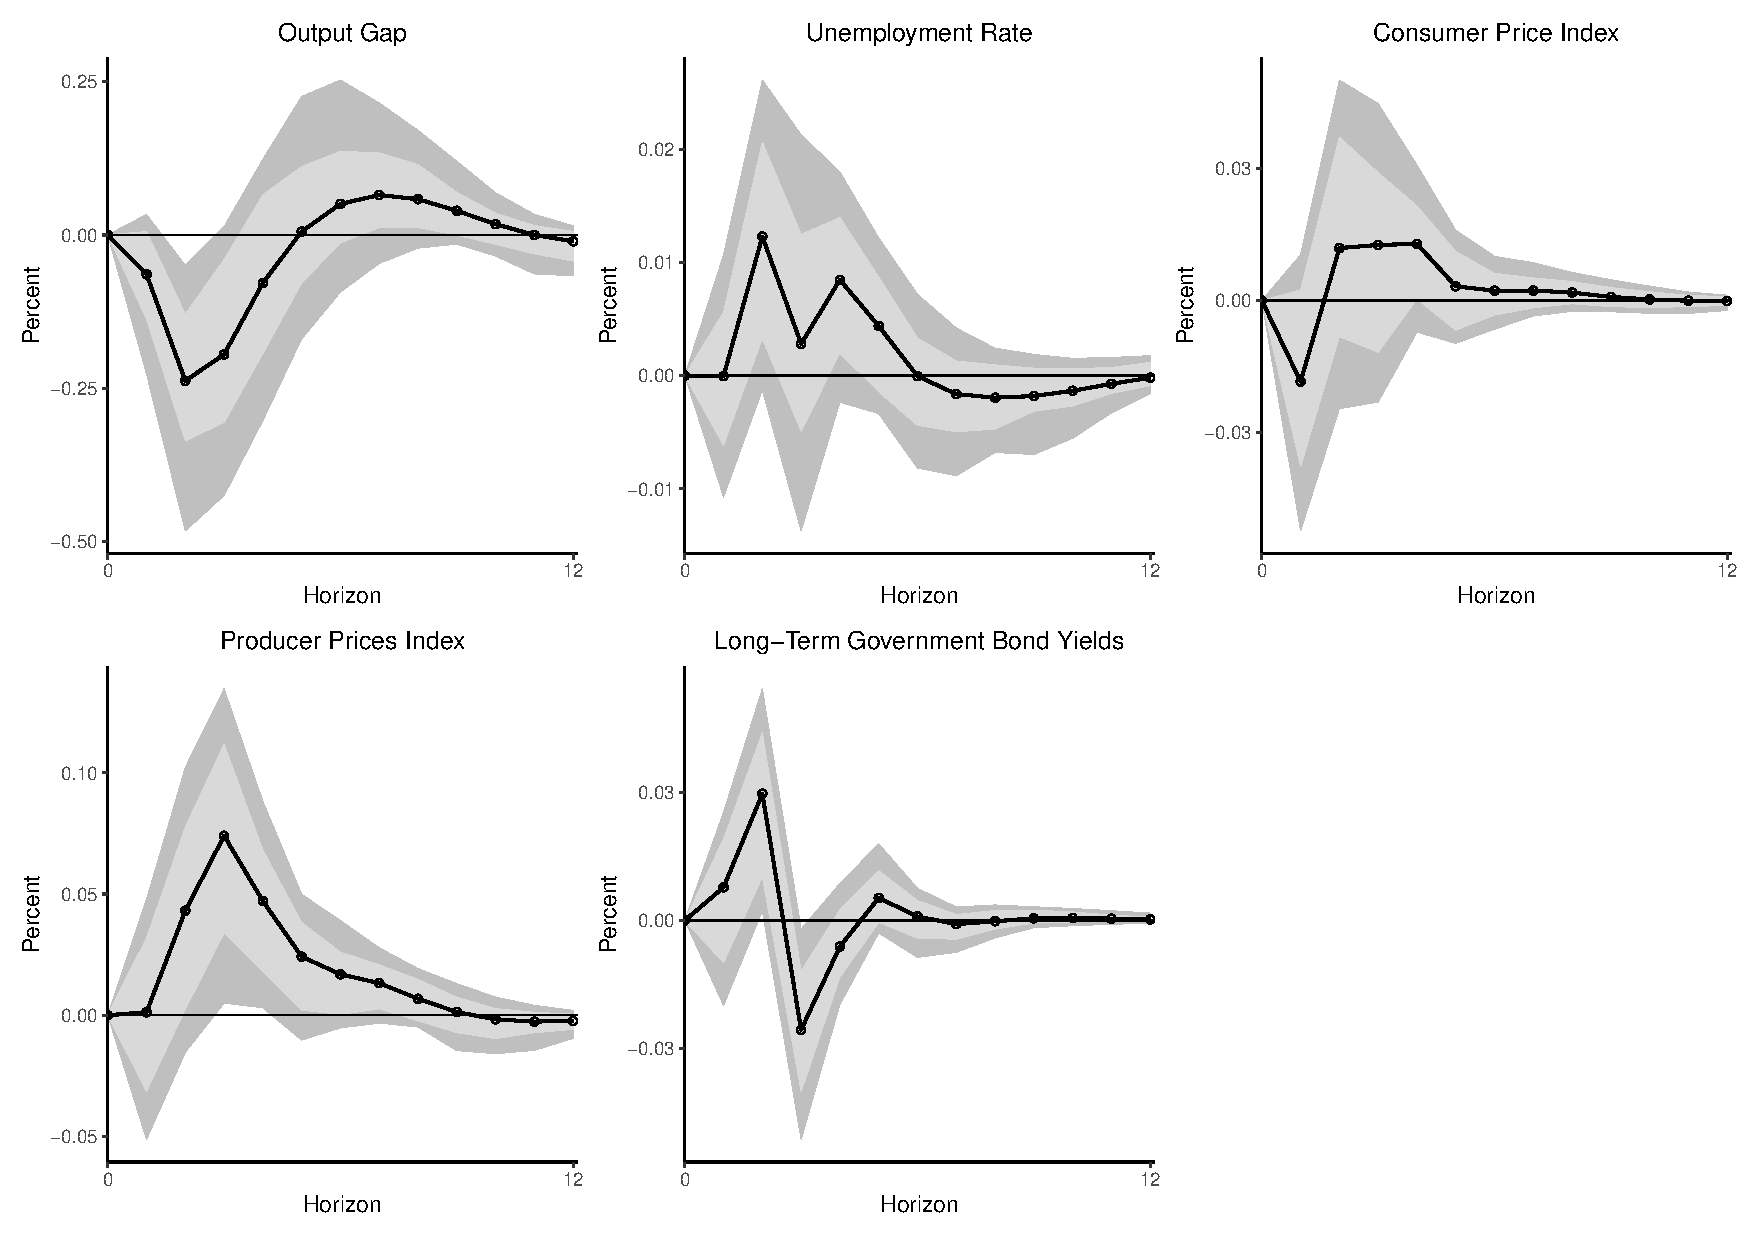
\includegraphics[width=\textwidth]{images/irf_vader.pdf}
    \caption*{Note: Impulse Response from a sentiment index shock (VADER). The variables are described as follows: Output gap -- obtained from a HP filter from Real Gross Domestic Product (Euro/ECU series) for Euro area; Unemployment Rate -- Harmonized Unemployment Rate: Total: All Persons for the Euro Area; Consumer Price Index -- Harmonized Prices: Total All Items for the Euro Area; Producer Prices Index -- Economic Activities: Total Industrial Activities for the Euro; and Long-Term Government Bond Yields: -- 10-year for the Euro Area. Following the literature, ``plotted are the point estimates, 68 (light grey), and 90 (dark grey) percent confidence bands'' \cite[p. 40]{shapiro2020measuring}.}
    \label{fig:my_label}
\end{figure}

\begin{figure}[!h]
    \centering
    \caption{Impulse Response of a Sentiment Index (LM-SA) Shock on Economic Activity}
    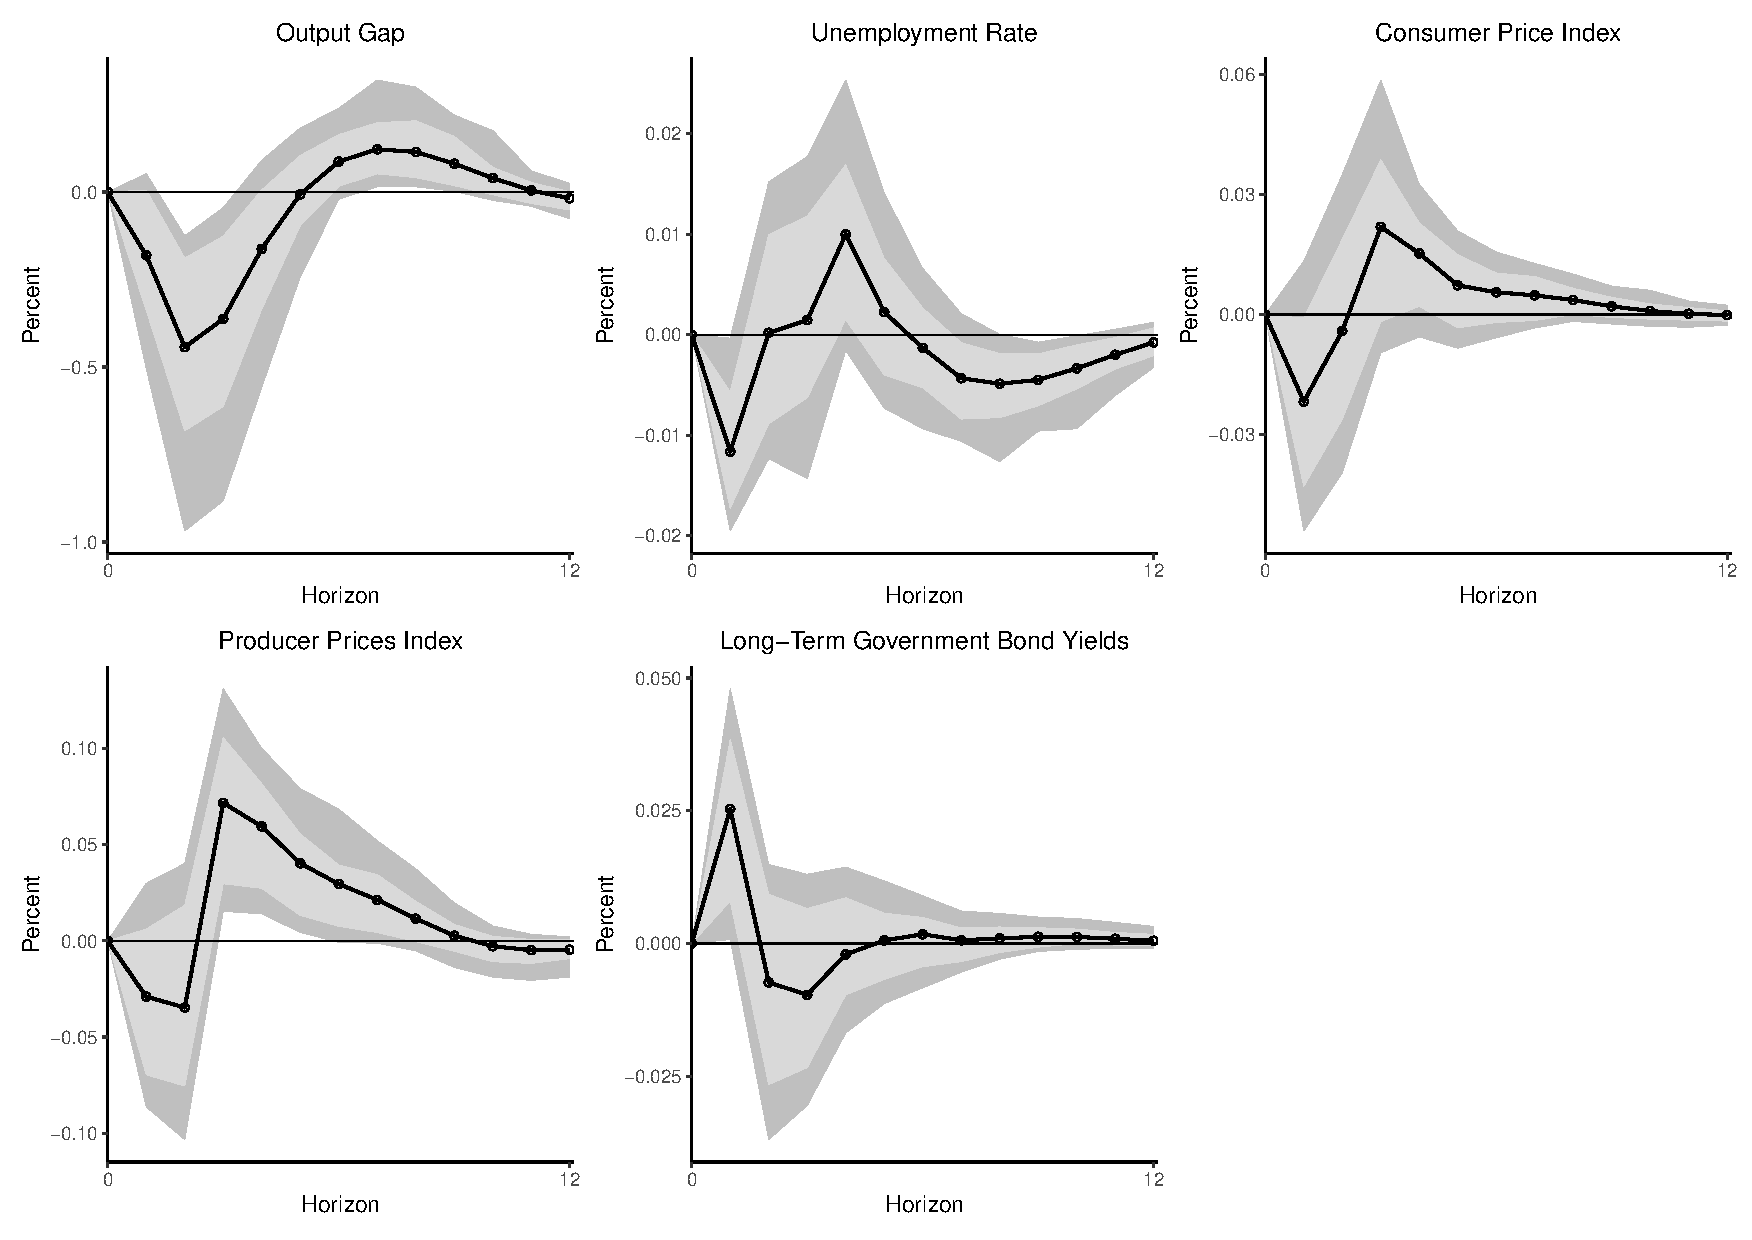
\includegraphics[width=\textwidth]{images/irf_lm.pdf}
    \caption*{Note: Impulse Response from a sentiment index shock (LM-SA-2020). The variables are described as follows: Output gap -- obtained from a HP filter from Real Gross Domestic Product (Euro/ECU series) for Euro area; Unemployment Rate -- Harmonized Unemployment Rate: Total: All Persons for the Euro Area; Consumer Price Index -- Harmonized Prices: Total All Items for the Euro Area; Producer Prices Index -- Economic Activities: Total Industrial Activities for the Euro; and Long-Term Government Bond Yields: -- 10-year for the Euro Area. Following the literature, ``plotted are the point estimates, 68 (light grey), and 90 (dark grey) percent confidence bands'' \cite[p. 40]{shapiro2020measuring}.}
    \label{fig:irflm}
\end{figure}

\subsection{Response of Economic Activity to Sentiment Indices}



\newpage


\section{Discussion}


